%
% pol-innen.tex
%
% (c) 2026 Damien Flury, OST Ostschweizer Fachhochschule
%
\begin{figure}
\centering
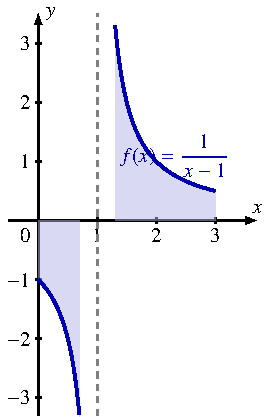
\includegraphics{papers/hauptwert/images/pol-innen.pdf}
\caption{Graph der Funktion $f(x)=1/(x-1)$ auf $[0,3]$.
Die Polstelle bei $x=1$ liegt im Innern des Integrationsintervalls;
symmetrische Annäherung mit gemeinsamem $\varepsilon$ liefert den Hauptwert.
\label{hauptwert:figure:pol-innen}}
\end{figure}
